% Source: Code/ML_overlay/ir_rgb_registration/paper/figures/fig_loss_architecture.tex
% Loss Function Architecture -- Affine Residual Loss (Experiment 3)
\documentclass[tikz,border=4pt]{standalone}
\usepackage[T1]{fontenc}
\usepackage{lmodern}
\usepackage{amsmath,amssymb}
\usetikzlibrary{arrows.meta,positioning,calc,fit,decorations.pathreplacing,backgrounds}

% Brand colors
\definecolor{Garnet}{HTML}{73000A}
\definecolor{Black90}{HTML}{363636}
\definecolor{Black70}{HTML}{5C5C5C}
\definecolor{Black50}{HTML}{A2A2A2}
\definecolor{Black30}{HTML}{C7C7C7}
\definecolor{Black10}{HTML}{ECECEC}
\definecolor{WarmGrey}{HTML}{676156}
\definecolor{Sandstorm}{HTML}{FFF2E3}
\definecolor{Rose}{HTML}{CC2E40}
\definecolor{Atlantic}{HTML}{466A9F}
\definecolor{Congaree}{HTML}{1F414D}
\definecolor{Horseshoe}{HTML}{65780B}
\definecolor{Grass}{HTML}{CED318}
\definecolor{Honeycomb}{HTML}{A49137}

\begin{document}
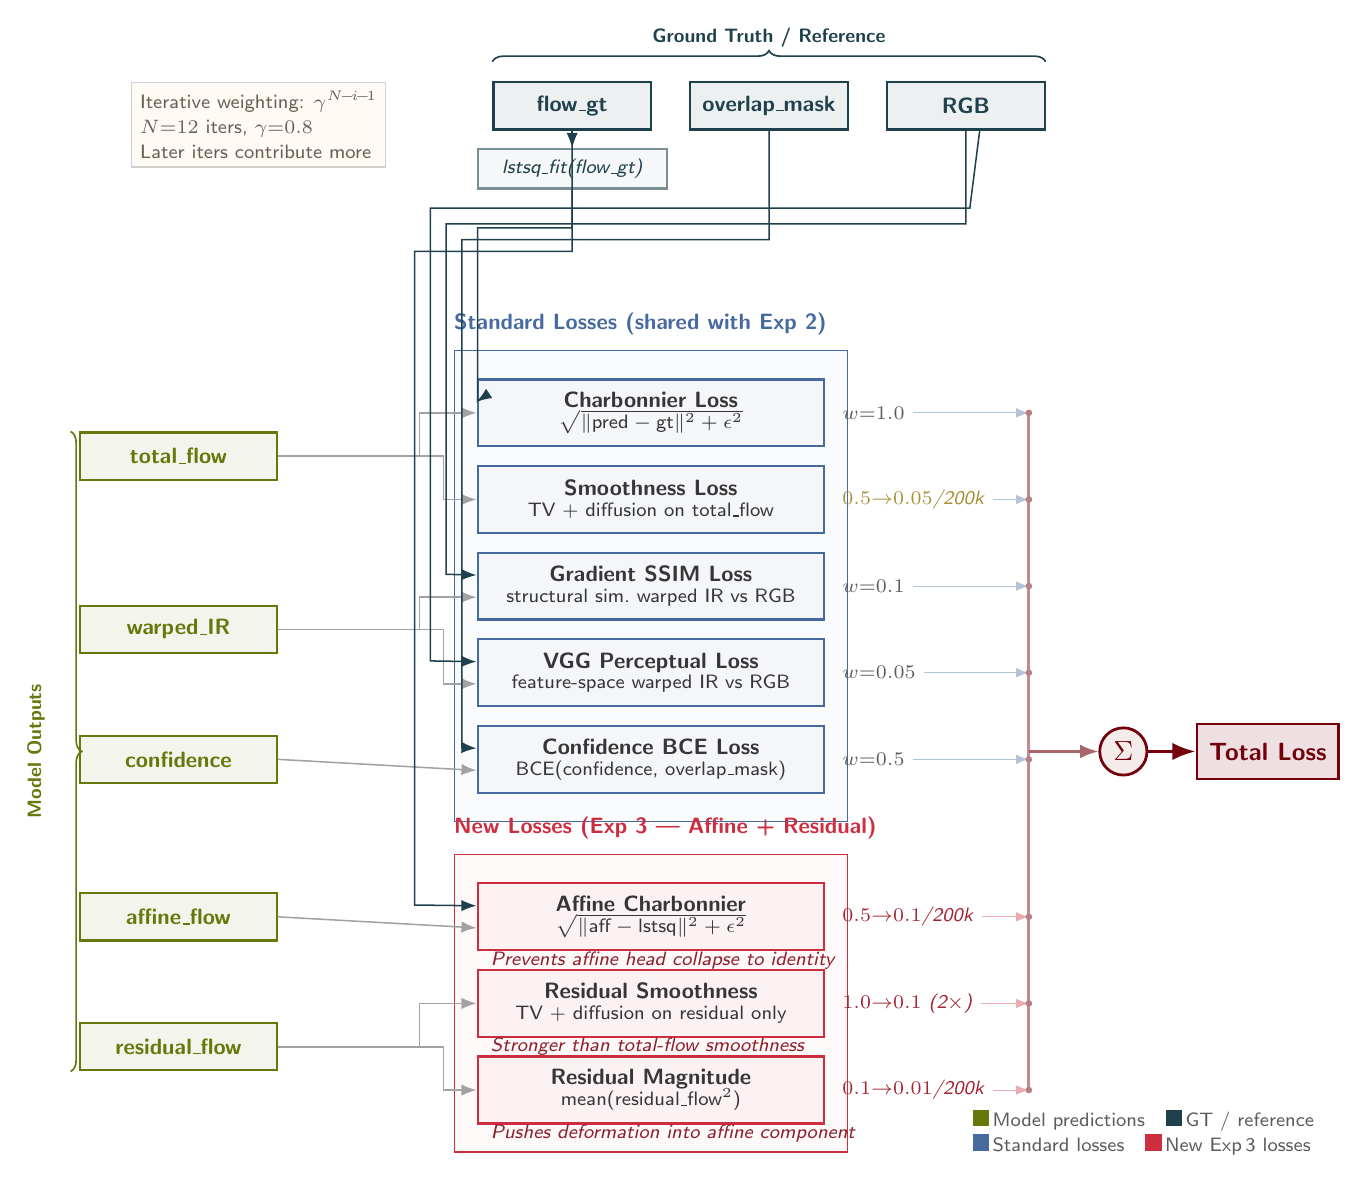
\begin{tikzpicture}[
    x=1cm, y=1cm,
    >=Latex,
    every node/.style={font=\sffamily\small, inner sep=0pt},
    pred/.style={
        draw=Horseshoe, fill=Horseshoe!8, line width=0.8pt,
        minimum width=2.5cm, minimum height=0.6cm,
        font=\sffamily\footnotesize\bfseries, text=Horseshoe,
        inner sep=3pt, align=center
    },
    gt/.style={
        draw=Congaree, fill=Congaree!8, line width=0.8pt,
        minimum width=2.0cm, minimum height=0.6cm,
        font=\sffamily\footnotesize\bfseries, text=Congaree,
        inner sep=3pt, align=center
    },
    stdloss/.style={
        draw=Atlantic, fill=Atlantic!6, line width=0.8pt,
        minimum width=4.4cm, minimum height=0.85cm,
        font=\sffamily\footnotesize, text=Black90,
        inner sep=3pt, align=center
    },
    newloss/.style={
        draw=Rose, fill=Rose!6, line width=0.8pt,
        minimum width=4.4cm, minimum height=0.85cm,
        font=\sffamily\footnotesize, text=Black90,
        inner sep=3pt, align=center
    },
    wlabel/.style={font=\sffamily\scriptsize, text=Black70, inner sep=1pt},
    anneal/.style={font=\sffamily\scriptsize\itshape, text=Honeycomb, inner sep=1pt},
    notetext/.style={font=\sffamily\scriptsize\itshape, text=Rose!70!black,
                     inner sep=1pt, align=left},
    dataarrow/.style={->, line width=0.55pt, color=Black50},
    gtarrow/.style={->, line width=0.55pt, color=Congaree},
    sumarrow/.style={->, line width=0.9pt, color=Garnet},
    bracestyle/.style={decorate, decoration={brace, amplitude=4pt, raise=2pt},
                       line width=0.6pt},
    groupbox/.style={draw=#1, line width=0.6pt, fill=#1!3, inner sep=5pt},
    grouplabel/.style={font=\sffamily\footnotesize\bfseries, text=#1},
    sumnode/.style={
        draw=Garnet, fill=Garnet!8, line width=1.0pt,
        circle, minimum size=0.6cm,
        font=\sffamily\normalsize\bfseries, text=Garnet, inner sep=0pt
    },
    totalloss/.style={
        draw=Garnet, fill=Garnet!12, line width=1.0pt,
        minimum width=1.8cm, minimum height=0.7cm,
        font=\sffamily\small\bfseries, text=Garnet,
        inner sep=3pt, align=center
    },
]

% =====================================================================
% LAYOUT PLAN
%
% x-coordinates:
%   -2.4 .. -0.1  Model predictions (center x=0, width=2.5cm)
%   1.8 .. 3.0    Prediction arrow routing lanes
%   3.0 .. 3.8    GT arrow vertical lanes (left of loss boxes)
%   3.9 .. 8.1    Loss boxes (center x=6.0, width=4.4cm so 3.8..8.2)
%   8.4+           Weight / schedule labels
%   10.8           Summation bus
%   12.0           Sigma node
%   13.5           Total Loss
%
% y-coordinates:
%   14.0           GT brace label
%   13.5           GT input boxes
%   12.7           lstsq_fit box
%   12.0           GT arrow horizontal routing level
%   11.4           "Standard Losses" label (above group box top ~11.2)
%   10.6           Charbonnier
%   9.5            Smoothness
%   8.4            Gradient SSIM
%   7.3            VGG Perceptual
%   6.2            Confidence BCE
%   5.8            Group box bottom (approx)
%   5.3            Gap between groups
%   4.9            "New Losses" label (above group box top ~4.7)
%   4.2            Affine Charbonnier
%   3.1            Residual Smoothness
%   2.0            Residual Magnitude
%   1.5            Group box bottom (approx)
% =====================================================================

\def\xloss{6.0}
\def\xbus{10.8}

% Standard loss y-positions
\def\yone{10.6}
\def\ytwo{9.5}
\def\ythree{8.4}
\def\yfour{7.3}
\def\yfive{6.2}

% New loss y-positions
\def\ysix{4.2}
\def\yseven{3.1}
\def\yeight{2.0}

% =====================================================================
% GT / REFERENCE INPUTS (top row) -- raised for clearance
% =====================================================================
\node[gt] (flowgt) at (5.0, 14.5) {flow\_gt};
\node[gt] (overlapmask) at (7.5, 14.5) {overlap\_mask};
\node[gt] (rgb) at (10.0, 14.5) {RGB};

% lstsq_fit derived from flow_gt
\node[gt, draw=Congaree!60, fill=Congaree!4,
      font=\sffamily\scriptsize\itshape, text=Congaree,
      minimum width=2.4cm, minimum height=0.5cm]
    (lstsq) at (5.0, 13.7) {lstsq\_fit(flow\_gt)};
\draw[gtarrow] (flowgt) -- (lstsq);

% =====================================================================
% STANDARD LOSSES (center column)
% =====================================================================
\node[stdloss] (charb) at (\xloss, \yone)
    {\textbf{Charbonnier Loss}\\[-2pt]
     {\scriptsize $\sqrt{\|\text{pred} - \text{gt}\|^2 + \epsilon^2}$}};

\node[stdloss] (smooth) at (\xloss, \ytwo)
    {\textbf{Smoothness Loss}\\[-2pt]
     {\scriptsize TV + diffusion on total\_flow}};

\node[stdloss] (gssim) at (\xloss, \ythree)
    {\textbf{Gradient SSIM Loss}\\[-2pt]
     {\scriptsize structural sim.\ warped IR vs RGB}};

\node[stdloss] (vgg) at (\xloss, \yfour)
    {\textbf{VGG Perceptual Loss}\\[-2pt]
     {\scriptsize feature-space warped IR vs RGB}};

\node[stdloss] (confbce) at (\xloss, \yfive)
    {\textbf{Confidence BCE Loss}\\[-2pt]
     {\scriptsize BCE(confidence, overlap\_mask)}};

% =====================================================================
% NEW EXP 3 LOSSES
% =====================================================================
\node[newloss] (affcharb) at (\xloss, \ysix)
    {\textbf{Affine Charbonnier}\\[-2pt]
     {\scriptsize $\sqrt{\|\text{aff} - \text{lstsq}\|^2 + \epsilon^2}$}};

\node[newloss] (ressmooth) at (\xloss, \yseven)
    {\textbf{Residual Smoothness}\\[-2pt]
     {\scriptsize TV + diffusion on residual only}};

\node[newloss] (resmag) at (\xloss, \yeight)
    {\textbf{Residual Magnitude}\\[-2pt]
     {\scriptsize mean(residual\_flow$^2$)}};

% =====================================================================
% WEIGHT / SCHEDULE LABELS (right of each loss, well clear)
% =====================================================================
\node[wlabel, anchor=west] (wcharb) at ([xshift=5pt]charb.east) {$w{=}1.0$};
\node[anneal, anchor=west] (wsmooth) at ([xshift=5pt]smooth.east) {$0.5{\to}0.05$/200k};
\node[wlabel, anchor=west] (wgssim) at ([xshift=5pt]gssim.east) {$w{=}0.1$};
\node[wlabel, anchor=west] (wvgg) at ([xshift=5pt]vgg.east) {$w{=}0.05$};
\node[wlabel, anchor=west] (wconfbce) at ([xshift=5pt]confbce.east) {$w{=}0.5$};

\node[anneal, anchor=west, text=Rose!80!black] (waffcharb)
    at ([xshift=5pt]affcharb.east) {$0.5{\to}0.1$/200k};
\node[anneal, anchor=west, text=Rose!80!black] (wressmooth)
    at ([xshift=5pt]ressmooth.east) {$1.0{\to}0.1$ (2$\times$)};
\node[anneal, anchor=west, text=Rose!80!black] (wresmag)
    at ([xshift=5pt]resmag.east) {$0.1{\to}0.01$/200k};

% =====================================================================
% MODEL PREDICTIONS (left column)
% =====================================================================
\node[pred] (totalflow)  at (0, 10.05) {total\_flow};
\node[pred] (warpedir)   at (0, 7.85) {warped\_IR};
\node[pred] (confidence) at (0, 6.2)  {confidence};
\node[pred] (affineflow) at (0, 4.2)  {affine\_flow};
\node[pred] (residflow)  at (0, 2.55) {residual\_flow};

% =====================================================================
% GROUP BOXES (background layer)
% =====================================================================
\begin{pgfonlayer}{background}
\node[groupbox=Atlantic,
      fit=(charb)(smooth)(gssim)(vgg)(confbce),
      inner xsep=8pt, inner ysep=10pt] (stdgroup) {};
\node[groupbox=Rose,
      fit=(affcharb)(ressmooth)(resmag),
      inner xsep=8pt, inner ysep=10pt] (newgroup) {};
\end{pgfonlayer}

% Group labels ABOVE group boxes with clear separation
\node[grouplabel=Atlantic, anchor=south west]
    at ([yshift=5pt]stdgroup.north west)
    {Standard Losses (shared with Exp 2)};
\node[grouplabel=Rose, anchor=south west]
    at ([yshift=5pt]newgroup.north west)
    {New Losses (Exp 3 --- Affine + Residual)};

% =====================================================================
% ARROWS: Model predictions --> Loss boxes (from left)
%
% Predictions route horizontally then vertically to loss box left edge.
% Uses staggered x-offsets so paths don't overlap.
% =====================================================================
% total_flow --> Charbonnier, Smoothness
\draw[dataarrow] (totalflow.east) -- ++(1.8,0) |- (charb.west);
\draw[dataarrow] (totalflow.east) -- ++(2.1,0) |- (smooth.west);

% warped_IR --> GSSIM, VGG (enter at bottom of left edge, offset from GT)
\draw[dataarrow] (warpedir.east) -- ++(1.8,0) |- ([yshift=-4pt]gssim.west);
\draw[dataarrow] (warpedir.east) -- ++(2.1,0) |- ([yshift=-4pt]vgg.west);

% confidence --> Confidence BCE (enter at bottom of left edge)
\draw[dataarrow] (confidence.east) -- ([yshift=-4pt]confbce.west);

% affine_flow --> Affine Charbonnier (enter at bottom of left edge)
\draw[dataarrow] (affineflow.east) -- ([yshift=-4pt]affcharb.west);

% residual_flow --> Residual Smoothness, Residual Magnitude
\draw[dataarrow] (residflow.east) -- ++(1.8,0) |- (ressmooth.west);
\draw[dataarrow] (residflow.east) -- ++(2.1,0) |- (resmag.west);

% =====================================================================
% ARROWS: GT / Reference --> Loss boxes
%
% ALL GT arrows route down the LEFT side of the loss column in
% vertical lanes between x=3.0 and x=3.8, entering loss boxes
% from the LEFT at specific y-offsets. This keeps the right side
% (weights, bus) completely clear.
%
% Lane assignments:
%   flow_gt:       drops at x=5.0 -> route at x=5.0 down to charb.
%                  Goes through the routing gap above the group box,
%                  straight into charb.north (no left-lane needed).
%   overlap_mask:  drops at x=7.5 -> routes at x=3.6 down to confbce
%   RGB (gssim):   drops at x=10.0 -> routes at x=3.4 down to gssim
%   RGB (vgg):     drops at x=10.0 -> routes at x=3.2 down to vgg
%   lstsq_fit:     drops at x=5.0 -> routes at x=3.0 down to affcharb
% =====================================================================

% Horizontal routing level (between lstsq and group box top, with clearance)
\def\yroute{12.8}

% flow_gt --> Charbonnier
% Drop to routing level, go left to lane x=3.8, drop to charb, enter left
\draw[gtarrow]
    (flowgt.south) -- (5.0, \yroute+0.15)
    -- (3.8, \yroute+0.15)
    -- (3.8, \yone+0.15)
    -- ([yshift=4pt]charb.west);

% overlap_mask --> Confidence BCE
% Drop to routing level, left to lane x=3.6, drop to confbce, enter
\draw[gtarrow]
    (overlapmask.south) -- (7.5, \yroute)
    -- (3.6, \yroute)
    -- (3.6, \yfive+0.15)
    -- ([yshift=4pt]confbce.west);

% RGB --> Gradient SSIM
% Drop to routing level (staggered +0.2), left to lane, drop, enter
\draw[gtarrow]
    (rgb.south) -- (10.0, \yroute+0.2)
    -- (3.4, \yroute+0.2)
    -- (3.4, \ythree+0.15)
    -- ([yshift=4pt]gssim.west);

% RGB --> VGG Perceptual
% Drop to routing level (staggered +0.4), left to lane, drop, enter
\draw[gtarrow]
    ([xshift=5pt]rgb.south) -- (10.05, \yroute+0.4)
    -- (3.2, \yroute+0.4)
    -- (3.2, \yfour+0.15)
    -- ([yshift=4pt]vgg.west);

% lstsq_fit --> Affine Charbonnier
% Drop to routing level, left to lane x=3.0, drop through gap to
% affcharb+offset, enter
\draw[gtarrow]
    (lstsq.south) -- (5.0, \yroute-0.15)
    -- (3.0, \yroute-0.15)
    -- (3.0, \ysix+0.15)
    -- ([yshift=4pt]affcharb.west);

% =====================================================================
% SUMMATION BUS (right side, past all labels)
% =====================================================================
\coordinate (bustop) at (\xbus, \yone);
\coordinate (busbot) at (\xbus, \yeight);

% Taps from weight labels to bus
\foreach \wnode/\col in {wcharb/Atlantic, wsmooth/Atlantic, wgssim/Atlantic,
                         wvgg/Atlantic, wconfbce/Atlantic,
                         waffcharb/Rose, wressmooth/Rose, wresmag/Rose} {
    \draw[\col!40, line width=0.35pt, ->]
        ([xshift=2pt]\wnode.east) -- (\wnode.east -| bustop);
}

% Bus line
\draw[Garnet!45, line width=1.0pt] (bustop) -- (busbot);

% Tap dots on bus
\foreach \ylev in {\yone, \ytwo, \ythree, \yfour, \yfive,
                   \ysix, \yseven, \yeight} {
    \fill[Garnet!50] (\xbus, \ylev) circle (1.2pt);
}

% Summation node
\node[sumnode] (sigma) at (12.0, 6.3) {$\Sigma$};
\draw[sumarrow, Garnet!60, line width=0.8pt]
    (\xbus, 6.3) -- (sigma.west);

% Total loss
\node[totalloss, right=0.6cm of sigma] (totloss) {Total Loss};
\draw[sumarrow, line width=1.2pt] (sigma) -- (totloss);

% =====================================================================
% ANNOTATION: Purpose notes (below each new loss box)
% =====================================================================
\node[notetext, anchor=west]
    at ([xshift=4pt, yshift=-5pt]affcharb.south west)
    {\raisebox{0pt}[0pt][0pt]{Prevents affine head collapse to identity}};
\node[notetext, anchor=west]
    at ([xshift=4pt, yshift=-5pt]ressmooth.south west)
    {\raisebox{0pt}[0pt][0pt]{Stronger than total-flow smoothness}};
\node[notetext, anchor=west]
    at ([xshift=4pt, yshift=-5pt]resmag.south west)
    {\raisebox{0pt}[0pt][0pt]{Pushes deformation into affine component}};

% =====================================================================
% ITERATIVE WEIGHTING NOTE (top-left)
% =====================================================================
\node[font=\sffamily\scriptsize, text=WarmGrey, align=left,
      anchor=north west, inner sep=3pt,
      draw=WarmGrey!30, fill=Sandstorm!40,
      minimum width=3.0cm]
    (iternote) at (-0.6, 14.8)
    {Iterative weighting: $\gamma^{N\!-\!i\!-\!1}$\\[1pt]
     $N{=}12$ iters, $\gamma{=}0.8$\\[1pt]
     Later iters contribute more};

% =====================================================================
% DECORATIVE BRACES
% =====================================================================

% Model outputs brace (left)
\draw[bracestyle, Horseshoe]
    ([xshift=-5pt]totalflow.north west) -- ([xshift=-5pt]residflow.south west)
    node[midway, left=7pt, font=\sffamily\scriptsize\bfseries,
         text=Horseshoe, align=center, rotate=90, anchor=south]
    {Model Outputs};

% GT inputs brace (top)
\draw[bracestyle, Congaree]
    ([yshift=5pt]flowgt.north west) -- ([yshift=5pt]rgb.north east)
    node[midway, above=7pt, font=\sffamily\scriptsize\bfseries,
         text=Congaree]
    {Ground Truth / Reference};

% =====================================================================
% LEGEND (bottom-right)
% =====================================================================
\node[font=\sffamily\scriptsize, text=Black70, align=left,
      anchor=south east, inner sep=2pt]
    at (14.5, 1.1)
    {\textcolor{Horseshoe}{\rule{6pt}{6pt}}\,Model predictions\quad
     \textcolor{Congaree}{\rule{6pt}{6pt}}\,GT / reference\\[1pt]
     \textcolor{Atlantic}{\rule{6pt}{6pt}}\,Standard losses\quad
     \textcolor{Rose}{\rule{6pt}{6pt}}\,New Exp\,3 losses};

\end{tikzpicture}
\end{document}
